%% 
%% ACS project dissertation template. 
%% 
%% Currently designed for printing two-sided, but if you prefer to 
%% print single-sided just remove ",twoside,openright" from the 
%% \documentclass[] line below. 
%%
%%
%%   SMH, May 2010. 


\documentclass[a4paper,12pt,twoside,openright]{report}


%%
%% EDIT THE BELOW TO CUSTOMIZE
%%

\def\authorname{From Context Embeddings to Meaning Embeddings \xspace}
\def\authorcollege{David Yenicelik \\ ETH Zürich\xspace}
\def\authoremail{yedavid@ethz.ch}
\def\dissertationtitle{}
\def\wordcount{14,235}


%\usepackage[dvips]{epsfig,graphics} 
\usepackage{epsfig,graphicx,verbatim,parskip,tabularx,setspace,xspace}
\usepackage{amsmath, amsfonts}
\usepackage{bbm}
\usepackage[ruled,vlined]{algorithm2e}


%% START OF DOCUMENT
\begin{document}


%% FRONTMATTER (TITLE PAGE, DECLARATION, ABSTRACT, ETC) 
\pagestyle{empty}
\singlespacing
% title page information
\begin{titlepage} 

\begin{center}
\noindent
\huge
\dissertationtitle \\
\vspace*{\stretch{1}}
\end{center}

\begin{center}
\noindent
\huge
\authorname \\
\Large
\authorcollege      \\[24pt]

\includegraphics{CUni3.eps}
\end{center}

\vspace{24pt} 

\begin{center}
\noindent
\large
{\it A dissertation submitted to the University of Cambridge \\ 
in partial fulfilment of the requirements for the degree of \\ 
Master of Philosophy in Advanced Computer Science} 
\vspace*{\stretch{1}}
\end{center}

\begin{center}
\noindent
University of Cambridge \\
Computer Laboratory     \\
William Gates Building  \\
15 JJ Thomson Avenue    \\
Cambridge CB3 0FD       \\
{\sc United Kingdom}    \\
\end{center}

\begin{center}
\noindent
Email: \authoremail \\
\end{center}

\begin{center}
\noindent
\today
\end{center}

\end{titlepage} 

\newpage
\vspace*{\fill}

\onehalfspacing
\newpage
{\Huge \bf Declaration}

\vspace{24pt} 

I David Yenicelik of ETH Zürich, being a candidate for the M.Sc. ETH in
Computer Science, hereby declare that this report and the
work described in it are my own work, unaided except as may be
specified below, and that the report does not contain material that
has already been used to any substantial extent for a comparable
purpose.

\vspace{24pt}
Total word count: \wordcount

\vspace{60pt}
\textbf{Signed}: 

\vfill

This dissertation is copyright \copyright 2020 David Yenicelik. 
\\
All trademarks used in this dissertation are hereby acknowledged.



\newpage
\vspace*{\fill}

\singlespacing
\newpage
{\Huge \bf Abstract}
\vspace{24pt} 

One of the goals of Natural Language Understanding \textit{NLU} is to formalize written text in a way, such that linguistic features can be captured through computational models, which can then again be used for downstream machine learning tasks.
The most popular methodology in NLU is the use of vectors that represent written text, including word-vectors, sentence-vectors, etc. 
These vectors are often referred to as \textit{embedding} vectors, as they embed more complex concepts into a vector representation.

Because embeddings - due to their strong usage in downstream tasks - can be considered as the fundamental unit of machine learning in the domain of natural language, any shortcomings will influence the performance of the target task.
Given that language models such as BERT only capture a black-box function $f$ between input and output, our aim is to understand how the subspace organization relates to linguistic features.
We focus our analysis on \textit{semantics}, which captures a meaning within language, as this is one of the most important features of language. 
We analyse the BERT language model, as it provides a good balance between popularity, close to state-of-the-art performance, and generalizability to other modern language models.
\\

Our main contributions are the following: (1) We test for linear separability and ability to partition the space into semantic clusters within the sampled BERT vectors.
We show that while linear separability is possible, it is nearly impossible to find modes in the data which correspond to semantic classes that are as cleanly as defined by WordNet.
We conclude that BERT organized the embedding vectors imminently by context, and very little by semantics alone.
This can easily introduce undesirable properties such as strong sentiment, leading to considerable bias in downstream tasks.
(2) We analyze the relationship between part-of-speech and semantics. 
We show that these show a strong correlation in languages and that modern language models capture this strong correlation.
This affects the conclusion of some related work which had analysed language models which capture semantics, but which did not account for the correlation between part-of-speech and semantics.
(3) Finally, we introduce additional parameters for words whose sampled embedding vectors have high variance over the embedding space.
We investigate what downstream tasks are most affected  and use this as a proxy to understand what information is captured the most by the directions with high variance. \\

\newpage
\vspace*{\fill}


\pagenumbering{roman}
\setcounter{page}{0}
\pagestyle{plain}
\tableofcontents
\listoffigures
\listoftables

\onehalfspacing

% Definition of macros
\newcommand{\norm}[1]{\left\lVert#1\right\rVert}
\newcommand{\bracket}[1]{\left[#1\right]}
\newcommand{\absdet}[1]{\left|#1\right|}
%% START OF MAIN TEXT 

%\chapter{Introduction}
\chapter{Introduction}
\pagenumbering{arabic} 
\setcounter{page}{1} 

In Natural Language Processing (NLP), bilingual lexical induction (BLI) is a problem of inferring word-to-word mapping between two languages.
While supervised BLI may be learned trivially from a dictionary, unsupervised BLI is highly non-trivial, and serves as a backbone to many unsupervised Neural Machine Translation (NMT) systems, without which the overall MT performance drastically drops \cite{dropping_perf1} \cite{dropping_perf2}.
In addition to the unsupervised setting, words in a source language A often do not carry a one-to-one correspondence with words in a target language B.
This further increases the difficulty of finding a (bijective) mapping between the two embedding spaces.

\section{Scope of Work}


Continuing where \cite{density_matching} left off, we want to investigate the performance of using normalising flows to model unsupervised lexicon matching between two probability distributions, which are defined by Gaussian emebddings, which have a one-to-one correspondence to tokens in the respective languages.
We aim to use Gaussian embeddings for the robustness, and better integration into the probabilistic perspective.
The method discussed in the paper also relies a lot on the (semi-)supervised loss component.
We aim to investigate why this is the case, and would like to revise a method which is more robust in the fully unsupervised setting.\\

\textbf{Minimal goals:} We propose the following steps on achieving this goal.


\begin{enumerate}
    \item Replicate the algorithms and models which can generate through Gaussian embedding \cite{gaussian_embedding}. Do one sanity check by doing a sanity check on one of (SimLex / WordSim)
    \item Replicate "Density matching for bilingual word embedding" to setup a baseline normalising flow between vector-word-embeddings \cite{density_matching}.
    \item Define loss between predicted and target embeddings (if change in definition is necessary)
    \item Change the embeddings in point 2. to use Gaussian embeddings. Implement Loss functions found in point 3.
\end{enumerate}

\textbf{Extended goals:} If the above points provide good performance , we would like to expand on the below points.

\begin{enumerate}
    \item Implement a fully unsupervised extension by investigating the shortcomings of \cite{density_matching}.
    \item Investigate "deeper" normalising flows than the linear flow in \cite{density_matching} as such \cite{flowpp} \cite{neuralsplineflow}.
\end{enumerate}


\textbf{Contingency Plan / Further extended goals:} Implementing the following points would allow for an applied perspective of this approach, showing that this methodology allows for more robust mapping, also outside the field of NLP.


\begin{enumerate}
    \item Train embeddings for job-systems ESCO and AUGOV using Skip-Gram or Co-Occurence-matrix based. Do a sanity check.
    \item Train Gaussian embeddings for job-systems. Do a sanity check.
    \item Generate a small validation dataset between the European- and Australian job-system.
    \item Setup some baseline algorithms based on NLP, graph-matching, colinear-PCA for matching as a non-NLP benchmark environment. Compare against above-proposed methods.
    \item Find a normlising flow model to transform one job system into another.
\end{enumerate}

TODO: Fill out at the very end!

\newpage
\chapter{Motivation}
 
- Natural Language Understanding (NLU) lies in the intersection of formalising human text into a computer-readable format.
- Computer-readble units must be numerical, thus we represent words and meanings by vectors
- The relationships between vectors should cover underlying relations between the word meaning
- Language models are a generalization of word vectors
- Word embeddings such as Word2Vec and language models such as BERT are used for other tasks, which are refered to as "downstream" tasks, due to their nature of using up these word-embeddings and language models

- Because these are the most basic units of text, any shortcomings and properties will propagate over to any downstream task
- Some properties include that static word vectors like word2vec form a bijection between discrete vectors and word tokens. 
However, because a single word can entail multiple meanings, such as the polysemous word "bank" ( (1) financial instution, (2) a sitting bench ), this results in a lossy compression
- Other language models like context embeddings entail too much information, and also include other linguistic features such as semantic information, relatenedness to unrelated concepts.
These properties can easily introduce bias into any downstream tasks.
- We conjecture that many language tasks incl. translation will benefit most from meaning information

- Our general approach is to start with a complex language model that outputs context embeddings, and find signals / vectors that entail meaning.
- Although this work is dedicated to the domain of natural language understanding, the principles analysed in this work should generalize to other domains with similar structural properties as well, where we want to denoise some embedding space to some select properties.


%\chapter{Background} 
\chapter{Background} 

TODO: Take some more from here
%TODO http://da.inf.ethz.ch/teaching/2019/CIL/lecture/CIL2019-05-Word-Embeddings.pdf

- Some of the main points behind \cite{harris54} are that there is inherent structure in language, and that this structure can be formalized.
- \cite{harris54} mentions that the relation between the linguistic representation in terms of sounds and tokens are related to the meaning that the representation entail.
- However, despite the obvious relationship, the distinction between distributional structure of the language and meaning is not always clear. and that there is a "parallel" meaning structure, and argues that there is not a one-to-one relation between vocabulary and classification of meaning. 
- Also argues that the meaning of a word is entailed by it's environment, and the words that it occurs with.
- Other viewpoints (CITE HOFMANNs "teachers") In the end, language captures the evolution of human thought.

- cite paper "meaning is classified by its context"

Chronologically, the following data structures are manifestations of the above idea of defining a word by it's neighborhood.

\section{Word Embeddings}

In general, we want to find a mapping 

\begin{equation}
w^t \mapsto w \in \mathbb{R}^{d}
\end{equation}

where $w^t$ is a token representation and where this token representation is transformed into a $d$-dimensional vector representation.

One of the early ideas of representing the distributional structure of words through a data structure was expressed in \cite{bengio03}. 

\cite{bengio03} argues that a statistical model of language can be represented by the conditional probability of the next word given all the previous ones.

\begin{equation}
\hat{P}\left(w_{1}^{T}\right)=\prod_{t=1}^{T} \hat{P}\left(w_{t} | w_{1}^{t-1}\right)
\end{equation}{\label{eq:previous_words}}

This is then relaxed using the markovian assumption that the future state is independent from the previous states given the current state.
Using this assumption, we arrive at the relaxed formulation of

\begin{equation}
\hat{P}\left(w_{t} | w_{1}^{t-1}\right) \approx \hat{P}\left(w_{t} | w_{t-n+1}^{t-1}\right)
\end{equation}

Another approach is to take a more global approach, and consider not only the preivous $t-1$ words, but the full context / neighrborhood of a word

\begin{equation}
\hat{P}\left(w_{1}^{T}\right)=\prod_{t=1}^{T} \hat{P}\left(w_{t} | w_{1}^{t-1}\right)
\end{equation}{\label{eq:previous_words}}

% REFACTOR

We want to use some rank-based Energy, not absolute energy, such that we can make sure that neighboring words are pushed together, and two "random" words are pushed further away from each other.

The above two problems can be regarded as finding an invertible transformation from one (embedding) space $\mathcal{X} \in \mathbf{R}^d$ into another $\mathcal{\hat{X}} \in \mathbf{R}^d$. 
Normalising flows \cite{variational_inference_using_normalized_flows} \cite{nvp} have proven to be a powerful tool in modeling such relations.
As such, the aim of this project is to find a model based on normalising flows which is able to find an an invertible mapping $f$ from $\mathcal{X}$ to $\mathcal{\hat{X}}$.
To keep the discussion focused, this thesis deals with the problem of finding a model for bilingual lexicon matching.

\subsection{Static Word Embeddings}

Static word embeddings are structural representations of words that for which each word token is represented by a vector, the so called \textit{word vector}.

\subsubsection{Word2Vec}

The most prominent example of word vectors manifests itself in the work of \cite{mikolov13}.
Here, a neural network with a single embedding layer can be trained to transform one-hot-vectors into a latent vector representation $w \in \mathbf{R}$.

The training procedure follows a \textit{continuous bag of words} methodology, or a \textit{continuous skip gram model}.
From experience, the skip gram model seems to be prevalent in the data science community. 

\begin{figure}
	\center
  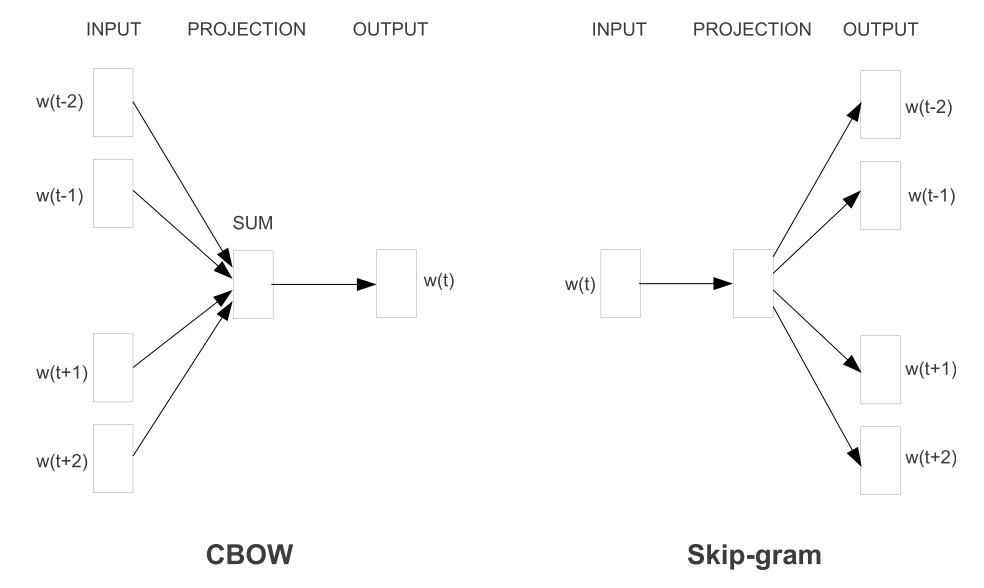
\includegraphics[width=0.6\linewidth]{./assets/background/cbow_and_skipgram.png}
  \caption{Figure taken from \cite{mikolov13}. The CBOW architecture predicts the current word based on the context. The Skip-gram predicts surrounding words given the current word.}
  \label{fig:boat1}
\end{figure}

Intuitively, this model is able to very well capture the idea of \cite{harris54} that the meaning of a word is captured by its neighborhood.

The underlying principle of \cite{mikolov13} is employed by the assumption that not only previous words, but the entire context of the word is taken into consideration when such a word vector is calculated.

However, other work argues that the context of a word is determined by its entire context.
In contrast to \eqref{eq:previous_words}, the underlying assumption can be represented as 

\begin{equation}
\hat{P}\left(w_{1}^{T}\right)=\prod_{t=1}^{T} \hat{P}\left(w_{t} | w_{1}^{t-1}\right)
\end{equation}

\subsubsection{GLoVe}

%TODO implement ETH slide equations

\subsubsection{Gaussian Embeddings}

Gaussian Embeddings have been first proposed in the context of words, although prior work has been adapted in embedding matrix-rows into a mean and standard deviation \cite{vilnis14} 

It is a continuous probabilistic relaxation of the otherwise common discrete point vectors.
Each word is represented by a Gaussian distribution in high-dimensional space, allowing to better capture uncertainty and a representation and it's relationships.
It can also express asymmetric relations more naturally than dot-products or cosine similarity, and enables for better-parametrized rule between decision boundaries.

Fitting Gaussian Mixture Models on embeddings have been done in order to apply Fisher kernels to entire documents.

Because this is an unsupervised learning task, we must use an energy function which is incorporated within a loss function that we try to minimize. 
The energy function describes (dis-)similarity between two items.
The authors propose the following energy functions to derive a Gaussian word-embedding.

\begin{equation}
L_m(w, c_p, c_n) = max(0, m - E_\theta(w, c_p) + E_\theta(w, c_n)
\end{equation}

Here, $w$ is the word we want to sample, $c_p$ is a "positive" context word, i.e. a word that co-occurs with the word $w$, and $c_n$ is a "negative" context word, i.e. a word that does not co-occur with the word $w$.
Usually the negative context words is sampled randomly from the corpus.
The loss function reminds of a hinge-loss in logistic regression.

The authors propose two possible ways to learn the mean and variance of the Gaussian embeddings.
They argue that the empirical covariance is not the most effective method of deriving the words as Gaussian embeddings.
This does not allow for inclusion between ellipsoids 

\paragraph{Symmetric similarity: expected likelihood or probability product kernel}

We can use any kernel (which is symmetric by definition) to derive at an energy function.
For two Gaussians $f(x)$, $g(x)$, the inner product is defined as:

\begin{align}
E_\theta(w, c) &= \int_{x \in \mathcal{R}^d} f(x)g(x) dx \\
&= \int_{x \in \mathcal{R}^d} \mathcal{N}(x; \mu_w, \Sigma_w) \mathcal{N}(x; \mu_c, \Sigma_c) dx \\
&= \mathcal{N}(0; \mu_w - \mu_c, \Sigma_w + \Sigma_c)
\end{align}

For numerical feasibility and easy of differentiation, we usually maximize the $\text{log} E_\theta(w, c)$ for a given dataset with $w \in \mathcal{W}, c \in \mathcal{C}$.
We will not go further in what the specific gradient of this log-energy is.

\paragraph{Asymmetric divergence: KL-Divergence}

We can use more directional supervision to exploit directional supervision, such as a knowledge graph.

Following energy-function is optimized:

\begin{align}
-E(w_i, c_j) & = D_{KL}(c_j || w_i) \\
&= \int_{x \in \mathcal{R}^d} \mathcal{N}(x; \mu_{w_i}, \Sigma_{w_i}) \text{log} \frac{\mathcal{N}(x; \mu_{c_j}, \Sigma_{c_j})}{\mathcal{N}(x; \mu_{w_i}, \Sigma_{w_i})} dx \\
&= \frac{1}{2}\left(\operatorname{tr}\left(\Sigma_{i}^{-1} \Sigma_{j}\right)+\left(\mu_{i}-\mu_{j}\right)^{\top} \Sigma_{i}^{-1}\left(\mu_{i}-\mu_{j}\right)-d-\log \frac{\operatorname{det}\left(\Sigma_{j}\right)}{\operatorname{det}\left(\Sigma_{i}\right)}\right)
\end{align}

Because of the loss function, this can entail information such as "y entails x" as a soft form of inclusion between two datasets (if KL divergence is used).
If a symmetric loss function is used, then this would most likely lead to overlap (IS THIS TRUE...???)

\paragraph{Uncertainty calculation:} In contrast to the empirical standard deviation as an uncertainty measure, we can now calculate the uncertainty of the inner product (i.e. the distribution $P(z=x^T y)$ using the following formula

\begin{align}
\mu_z = \mu_x^T \mu_y
\Sigma_z = \mu_{x}^T \Sigma_{x} \mu_{x}+\mu_{y}^T \Sigma_{y} \mu_{y}+\operatorname{tr}\left(\Sigma_{x} \Sigma_{y}\right)
\end{align}

We then get an uncertainty bound, where $c$ denotes the number of standard deviations away from the mean.
\begin{equation}
\mu_{x}^{\top} \mu_{y} \pm c \sqrt{\mu_{x}^{\top} \Sigma_{x} \mu_{x}+\mu_{y}^{\top} \Sigma_{y} \mu_{y}+\operatorname{tr}\left(\Sigma_{x} \Sigma_{y}\right)}
\end{equation}

We can learn the parameters $\Sigma$ and $\mu$ for each of these embeddings using a simple gradient-based approach, where we set hard constraints on 

\begin{align}
& \norm{ \mu_i }_2  \leq C, \forall i \\
& m I <  \Sigma_i < M I
\end{align}

The method shows competitive scores to the Skip-Gram model, although usually only with minor improvements depending on the benchmark-dataset.


\subsection{Context Embeddings}

\subsubsection{The Transformer Architecture}

All of the below presented models use the transformer architecture (cite the paper "attention is all you need!")

\subsubsection{ELMo}

\subsubsection{BERT}

\subsubsection{GPT and GPT-2}



\subsection{Other methods}

Although the above presented methods are the prevailent methods for word-embeddings, there are also other methods which do not clearly fit into one of the above categories.

\subsubsection{Generating "static" word-embeddings through contextual embeddings}

Some work has been done in extracting word-embeddings from contextual language models like BERT or ELMo.

CITE (BERT WEARS GLOVES: DISTILLING STATIC EMBEDDINGS FROM PRETRAINED CONTEXTUAL REPRESENTATIONS)

(1) Uses \textit{pooling} between BERT tokens to arrive at a single representation between words.

Here, sentences are split by space (tokenized).
Words are tokenized further into a subword as defined by WordPiece (Wu et al. 2016).

The defined pooling operations looks as follows to arrive at the word from the individual subwords:

$$
\mathbf{w}_{c}=f\left(\mathbf{w}_{c}^{1}, \ldots, \mathbf{w}_{c}^{k}\right) ; f \in\{\min , \max , \text { mean, last }\}
$$

where we have subwords $w^{1},  \ldots, w^{k}$ such that $\operatorname{cat}\left(w^{1}, \ldots, w^{k}\right)=w$

Why would any of these pooling operations result in a meaninigful source-word? 
This is just squishing tokens together! \\

-> This is a major limitation for which we may need to use ELMo
-> However this may be needed for "unseen concepts" (which are unseen words...)
-> Perhaps check what fasttext does...?


(2) Uses \textit{context combination} to map from different contexts $c_1, \ldots, c_n$ to a single static embedding $w$ that is agnostic of context.

Proposed are two ways to represent context.

\textbf{Decontextualization} For a single word-context, we siimply feed-in the word by itself to the model.

\textbf{Aggregated} combine $w$ in multiple contexts.
n sentences are sampled from the dictionary $\mathcal{D}$.
From the multiple sampled words, we then apply pooling to arrive at a single representation that aggregates the different tokens into one.

$$
\mathbf{w}=g\left(\mathbf{w}_{c_{1}}, \dots, \mathbf{w}_{c_{n}}\right) ; g \in\{\min , \max , \text { mean }\}
$$


This post extracts (token?) word-embeddings: 
(https://towardsdatascience.com/nlp-extract-contextualized-word-embeddings-from-bert-keras-tf-67ef29f60a7b)

This seems to be a way to extract embeddings for tokens from BERT
(https://github.com/imgarylai/bert-embedding)

(->How can we create a (parametric) probability density from a point-cloud distribution?)

perhaps not necessarily interpretable in standard euclidean space
(https://www.kdnuggets.com/2019/02/bert-features-interbertible.html)
original (https://medium.com/thelocalminima/are-bert-features-interbertible-250a91eb9dc)

Perhaps we can mask all but the target token to arrive at one vector per token (and then combine them somehow...).
But how do they extract the singular word-embeddings...?

(-> you could be like "acquiring bedeutung" is a big problem in many tasks. especially useful when we try to map one concept to another. we look at the NLP task for concreteness)

Generally, really good critique on this paper:

(https://openreview.net/forum?id=SJg3T2EFvr)

usually, we have sentence-embeddings, and do not look at word-embeddings.

(-> we don't want to add more and more context. we want a model which contains the polysemy of different contexts, which could allow for probability maximization..., otherwise we have to look at bigger and bigger documents to build more accurate language models, which becomes infeasible at some point. (although this would be the way humans work, because they live in context as well)

This blog aims to generate word-embeddings (and sentence-embeddings) from the BERT model.
(https://mccormickml.com/2019/05/14/BERT-word-embeddings-tutorial/)

create word-vectors by taking out what BERT predicts at the nth token.
create word-vectors by concatenating or summing multiple layer's outputs.

the cosine similarity between these vectors seem pretty well-done!


(-> Does it make sense to use BERT and then on calculate word-embeddings through an extended fully-connected model)

-> ELMo may provide a better tokenizer, maybe better ot use this? What about GPT? ELMo uses moses tokenizer which seems word-level enough

-> How to solve this tokenization problem....

-> Can also analyze only words that exist.




\chapter{Related Work}

\section{Structure inside BERT}

(How Contextual are Contextualized Word Representations? Comparing the Geometry of BERT, ELMo, and GPT-2 Embeddings)

going down the drain of "geometry" of BERT and ELMo.

could also go down the drain of bias (we would prefer to have uniform space over gender etc.)

-> does projection into some subspace which has same metric properties perhaps not make it asitropic?

pretty ok summary of what kind of properties we want from word-embeddings... (https://devopedia.org/word-embedding)


Especially in Named Entity Recognition (NER), there is a lot of use for static word-embeddings.
I guess this is because we need static embeddings which represent the individual clusters?

-> Using pooling for some 

-> Character level operation

-> Perhaps make good sense to work towards a word-embeddings where different vectors are close to each other?

-> perhaps find a metric space warping the vectors, s.t. an isotropic representation is achieved?

-> Perhaps tokenization is a big problem, but perhaps other architecture..? but retraining is too difficult.. probably best to just stick to BERT? one way or the other, we need good word-embeddings derived from good language models to form a probabilistic prediction of the concept


-> Could perhaps also try to make an adversarial autoencoder after the BERT layer (or continue training, s.t. a second loss is mimized as a downstream task?)

-> Perhaps distilling with "correct" tokens? i.e. another network which copies BERT, but instead of outputting \#\#end, it outputs one of most frequent 20k words

-> thesaurus using a (set of) words. a little like sentence-generation, but generating most-probable examples

-> Everyone just averages token-embeddings..

-> perhaps fitting a GMM to the contextualized representations of BERT may give a good probability space..?

-> Perhaps make sense to apply MUSE to this?

-> Artetxe 2019 uses language models to generate embeddings. we also do this, but do it using 1) better language models, and 2) better 

-> QUESTION: Which factors (mapping algo, embedding) is delimiting in automated embedding matching

-> perhaps create a GMM for each concept, based on how many modals we identify? how to estimate the number of clusters? by graph-clustering perhaps! (this could be very consuming)

-> Adversarial autoencoder on BERTs last models to enforce it to some better distribution

\section{Metric Learning and Disentanglement}

\section{Zero shot and One shot learning }

\section{Clustering Algorithms}

\section{Applications of word vector}




















































\newpage
\subsubsection{Word2Vec}

BERT conditions on the rest of the input sentence.

BERT uses words, subwords and individual characters (in total 30'000) that are then used as tokens.

Idea is to do the following:
Concepts (and thus words), are represented across multiple contexts.
We can create probabilistic word-embeddings by sampling from a corpus the context of a specific word.
From multiple samples of the context-embedding-vector, we take the mean and stddev, or create a GMM if there are multimodal logic (we can check this multimodality by runniing some sort of rejection sampling algorithm).
Then we have a probability density function (one for each language), and can map one into another.

Perhaps we could split up too high-variance embeddings to multimodal embeddings, depending on their use-cases.

This allows for interpretability in polysemy sentences.

Not using more complex flows implies that the flow itself is not the bottleneck (they probably tried out other flows as well).

Are the individual word-embeddings going to be one big blob with high variance, or is it going to be a multi-modal distribution...?

Another task we may look at is, from a given word-embedding, sample it's context. 
Not entirely sure how to do this with BERT and co.

At what point do we overfit, and at what point do we generalize?


\textbf{Artetxe bilingual token matching through unsupervised machine translation}

- Input is cross-lignual word-embeddings
- Build an unsupervised phrase-based statistical machine translation system
- Derive phrase-based embeddings from input-word-embeddings by taking top 400'000 bigrams and 400'000 trigrams -> take arithmetic mean of word-embedding
- score top 100 close phrases using softmax cosine similarity
- generation of synthetic parallel corpus using this approach
- Then use FastAlign to use parallel corpus to align words
- 

%\chapter{Related Work} 
\chapter{Related Work}

As outlined by (https://ruder.io/cross-lingual-embeddings/) the task of finding cross-lingual embedding models fall within one of the four categories:

\begin{enumerate}
\item Monolingual mapping: Here we train the embedding for each language separately, and the try to find a mapping from one space into another.
The learned mapping is usually linear.
\item Pseudo-cross-lingual: Here, a pseudo-language is created by mixing corpus from different languages.
The cross-lingual context is used to learn the shared embedding space.
[To what extent is this applicable?]
\item Cross-lingual training: parallel corpus used to train combined embeddings. Similar words will be mapped close to each other in same embedding space.
\item Joint optimization: Optimizing a combination of cross-lingual and monolingual losses.
\end{enumerate}

For parallel data, we can have different types of data:

\begin{enumerate}
\item Word-aligned data
\item Sentence-aligned data
\item Document aligned data
\item Lexicon (translations between multiple language-tables)
\item No parallel data (only monolingual resources)
\end{enumerate}

These are the ways to train word-embeddings (amongst others):

\begin{itemize}
\item word2vec variants
\item skip-gram with negative sampling (SGNS)
\item continuous bag-of-words (CBOW)
\item GloVe matrix factorization approach
\end{itemize}

Learning a linear projection from monolingual embeddings and parallel data.

Projection via CCA (Canonical component analysis).
A transformative matrix is learned for each language, the mapped space is the same space across different languages.
Using 80\% of projection vectors and using top k components generally yield highest performance.

Normalisation and orthogonal transport.
Product similarity measure (correlation) can be seen as Wasserstein distance (because it measures how much data points are away from each other) $c^Tc$.
Vectors are normalised during training with unit vector.
Because unit length, we can solve this by an orthogonal matrix.
(Does any information go away? Maybe it's good to regualrize even further so that we know that the mapping is indeed possible?)

Max-margin intrudercs.
Linear least squares leads to the hubness problem. 
Words tend to appear as nearest neighbors of many other words
(-> perhaps some non-random sampling is best here? to move away).
Use a ranking loss (sounds like optimal transport again...)
Ranking loss is also used in wasserstein context.

Alignment based projection:
Count number of times each word in source language is aligned with each word in target language document / sentence.

Adversarial autoencoder
Autoencoder learns to re-create the embedding, while discriminator learns to maximize the projection

Orthogonal transformation, normalisation, mean centering
Relation between the constraints is not clear.
Starting with basic optimization objective, they add regualizers and loss functions as intuitively make sense.
-> Dot-products need to be maintained after the mapping (as much as possible) constraint ( i dont like )
-> equal contribution to objective done by normaliizing the embedding..
-> two randomly selected words should in general not be similar

\paragraph{Pseudo-Cross-Label}
Captures interactions between words in different languages.
Mostly skipped because brain capacity...

Joing training with 2 x 2000 dimensional input (one for each job-system)... can then translate each one in one latent space to another.
How do we find parallel logic here, however..?


(-> Perhaps it makes sense to draw all the literature in the context of wassetstein, to do a probabilistic and principled analysis from there on.)








Observation (FRAGE: Frequency-Agnostic Word Representation): It is a feature that most-frequent words are embedded to different locations than non-most-embedded features.
Xing et al argue there is a mismatch between the way it is learned, and the projection and loss-function.
Tries to find a uniform theory across the three components.






If we use monolingual resources only, the common approach is

I focus on work which solely includes as input the bilingual word-embeddings.
Because I want to devise an algorithm which can map from any "matrix column" to any other "matrix column" (i.e. token to token, or item to item), I will not include papers which take as input NLP sentences / corpora used to build the embeddings. 

This work deals with some summary on how unsupervised bilingual lexicon matching was achieved in past papers.

I will give a short summary of papers sorted by year of appearance, and what additional contributions and observation were added since the last iteration.

Some terminiology before we start

\paragraph{online data} implies that some sort of parallel corpora is available
\paragraph{offline data} implies that we use pre-trained monolingual embeddings to arrive at a toen-translation task

The general goal of bilingual lexicon matching is to learn a shared embedding space where words possessing simiilar meanings are projected to nearby points.

Most existing methods focus on minimizing the distance between the two token-datasets using some (variation) of Wassterstein, Jensen-Shannon divergence, etc.

What are datasets that we can use for benchmarking

\begin{itemize}
\item MUSE dataset (as used in Zhou 2019 et al
\item 
\end{itemize}

Instead of mapping one system into another, we can also allow for joint-training of the word-embeddings.

(This resource is great!!!
https://ruder.io/cross-lingual-embeddings/
)





\section{Discrete Methods }

\subsection{Loss in Translation}

Finding a non-orthogonal mapping is more effective, especially with distance dictionaries

Orthogonality preserves distances between word-pairs.

Euclidean closest nearest neighbor is taken as the translation pair.

Hubs are words that appear too frequently close to other words.
This retrieval criterion suffers from the hubness problem.

Removing the loss creates a discrepancy between inference and training.

(-> Why should a loss-function be symmetric, not be symmetric?)

(-> especially with chinese. perhaps the non-orthogonality captures the ambigious tokens..?)

From the original problem of finding an orthogonal projection, we assimilate the auxiliary problem of

the CSLS criterion looks as follows:

\begin{equation}
CSLS(x, y) = - 2 \text{cos}(x, y) + \frac{1}{k} \sum_{\mathbf{y}^{\prime} \in \mathcal{N}_{Y}(\mathbf{x})} \cos \left(\mathbf{x}, \mathbf{y}^{\prime}\right)+\frac{1}{k} \sum_{\mathbf{x}^{\prime} \in \mathcal{N}_{X}(\mathbf{y})} \cos \left(\mathbf{x}^{\prime}, \mathbf{y}\right)
\end{equation}

We then use the objective function of a relaxed 

\begin{align} 
\min _{\mathbf{W} \in \mathcal{O}_{d}} \frac{1}{n} & \sum_{i=1}^{n}-2 \mathbf{x}_{i}^{\top} \mathbf{W}^{\top} \mathbf{y}_{i} \\+& \frac{1}{k} \sum_{\mathbf{y}_{j} \in \mathcal{N}_{Y}\left(\mathbf{W} \mathbf{x}_{i}\right)} \mathbf{x}_{i}^{\top} \mathbf{W}^{\top} \mathbf{y}_{j} \\+& \frac{1}{k} \sum_{\mathbf{W} \mathbf{x}_{j} \in \mathcal{N}_{X}\left(\mathbf{y}_{i}\right)} \mathbf{x}_{j}^{\top} \mathbf{W}^{\top} \mathbf{y}_{i} 
\end{align}

The optimization is over a convex manifold.



\subsection{MUSE Facebook using a Min-Max objective}

CSLS used in the training objective directly instead of using it just during retrieval.

Mikolov et. al learn a mapping between the two sets of $Y$ and $X$:

\begin{equation}
W^{\star} = \text{argmin}_{W \in M_d(\mathbf{R})} \norm{WX - Y}_F
\end{equation}

Translation of any source token $s$ to a target token $t$ is defined as 

$$
t = \text{argmax}_t \text{cos} (Wx_s, y_t)
$$

(i.e. we just create a mapping between $x$ and $t$ using a linear interpolation matrix and take the maximal scalar product.

Mikolov et al do not observe improved loss when using more advanced neural networks..

Enforcing an orthogonality constraint, this boils down to the procrustes problem as given by

\begin{equation}
W^\star = \text{argmin}_{W \in O_d(\mathbf{R}) } \norm {WX - Y}_F = UV^T 
\end{equation}

where $U$ and $V^T$ respectively the left and right Eigenvectors of $YX^T$.

We can create an adversarial unsupervised approach by taking random samples from 

$ X = \{ x_1, \dots, x_n \} $ and $ Y = \{ y_1, \dots, y_m \} $

where the discriminator has to detect which of the two datasets the sample stemmed from.
The "generator" (not really a generator) $W$ is trained to prevent the discriminator from making accurate decisions.
Specifically, this is modeled as a two-player game, where $WX$ and $Y$ should be as similar as possible.

As such, the discriminator objective is: 

\begin{align}
\mathcal{L}_D(\theta_D | W) &= \\ 
&= -\frac{1}{n} \sum_{i=1}^n \text{log} P_{\theta_D}  (\text{source} = 1 | W x ) \\ &-  \frac{1}{m} \sum_{i=1}^n \text{log} P_{\theta_D}  (\text{source} = 0 | W x )
\end{align}

and the generator objective is:

\begin{align}
\mathcal{L}_W(W|\theta_D) &= \\
&= -\frac{1}{n} \sum_{i=1}^{n} \log P_{\theta_{D}}\left(\text { source }=0 | W x_{i}\right) \\ 
&-  \frac{1}{m} \sum_{i=1}^{m} \log P_{\theta_{D}}\left(\text { source }=1 | y_{i}\right)
\end{align}

Here, the discriminator is trained on the labels whether the word came from the first embedding, or the second embedding.

(-> Is there a mathematical way to simply this..?)

The resulting rotation matrix is not on-par with supervised approaches.
As such, the authors propose to make use of the frequencies as additional information.
As such, we use the most common words as anchors.

We then generate a dictionary from the two embeddings.
Then we solve the procrustres to arrive at the final orthogonal matrix.

Use of the CSLS













\section{Methods using Normalising Flows}

\subsection{Density Matching for Bilingual Word Embeddings (Zhou 2019)}

Zhou et. al consider the problem by creating two smooth embedding spaces.

For simplicity, I will refer to embedding space $\mathcal{X} \in \mathbf{R}^d$ as the source embeddings, and the embedding space $\mathcal{Y} \in \mathbf{R}^d$ as the target embeddings. 

We denote $ x_i $ and $y_j$ as the individual words with respective embeddings $x \in \mathcal{X}$ and $y \in \mathcal{Y}$.

--------

The general approach of the authors is as follows:

We learn two mapping functions $f_{xy} : \mathcal{X} \rightarrow \mathcal{Y}$, $f_{yx} : \mathcal{Y} \rightarrow \mathcal{X}$

We maximize the density of data points in the source space. 
We use a log-likelihood term in the loss-function.

For monolingual embeddings, we define tractable density functions $p(x)$, $p(y)$.

We use gaussian embeddings, where each single gaussian module represents a single word.

\begin{equation}
p(x) \approx p(y) \approx GMM
\end{equation}

This implies that for both $\forall x \in \mathcal{X}$ and $\forall y \in \mathcal{Y}$ we have

\begin{equation}
p(x) = \sum_{i \in {1, \ldots, N_x} } \pi(x_i) \tilde{p}(x|x_i)
\end{equation}

where the final probability term $$\tilde{p}(x|x_i) = \mathcal{N}(x | x_i, \sigma^2_x I) $$ describes the probability density of the single word-embedding, represented through a Gaussian in this case, and $N_x$ defines the total number of components / words in dictionary $\mathcal{C}$.

To initiate the embeddings, the authors use the word2vec (WAS IT WORD2VEC) point-vector as the mean of the Gaussian distribution, and use a fixed variance term $\sigma^2$ for all Gaussians.

Furthermore, instead of using a uniform prior over the mixture weights $\pi(x_i)$, the authors use the observation that frequencies may give bettern information, as as such initiate the priors as the relative frequencies of the words, i.e. $$ \pi(x_i) = \frac{ \text{freq} (x_i) }{\sum_j \text{freq} (x_j) } $$ .

This implies that the experiment is not executed in a manner where the Gaussian Mixutres are carefully chose, but rather by augmenting and generalizing the word2vec point vectors to Gaussian distributions.
This has the effect that the resulting probability space becomes smooth (rather than a discrete space of point-vectors) [CITE??? SMOOTHNESS]
Another assumption made is that a gaussian distribution is best-able to capture this mixtures.

--------

Every training step obtains samples form the Gaussian mixture space.

The density calculation can be defined by using volume-preserving invertible transformations. 
Perhaps it could make sense to also apply convolutional operators?

To stabilize the unsupervised training, the author employs the following methods.

\begin{enumerate}
\item back-translation-loss to train both directions (this is conceptually similar to the cyclic dependency in GANs.
\item  the author uses a weakly loss. identical text-strings in both languages are mapped to similar places in the space. 
\item frequency of the words is used as a prior to the GMM prior weights.
\end{enumerate}

The authors indicate robust training which is not strongly dependent on initialization


------

The training functions in such as a way as to increase the log-probability density.
The general approach is:

\begin{enumerate}
\item A continuous vector $x$ is sampled from the GMM. 
Specifically,
\begin{equation}
x_i \sim \pi(x_i), x \sim \tilde{p}(x|x_i) 
\end{equation}
\item We then apply $f_{xy}$ to get the inferred target embedding $y = f_{xy}(x)$.
Specifically, we define the mapping operation as: 
\begin{equation}
f_{xy}(\cdot) = W_{xy} \cdot
\end{equation}
We choose $W$ as an invertible matrix, thus, the inverse function is defined as 
\begin{equation}
x = f(y) = W_{xy}^{-1} y
\end{equation}
setting the volume of this operation to $$ J(f^{-1}(x)) = W_{xy} $$ which is used for the log-density calculations.
Specifically
\begin{equation}
\text{log} p(x; W_{xy}) = \text{log} p(y) + \text{log} \absdet{\text{det}(W_{xy})}
\end{equation}
\item We then maximize the log-likelihood, which equivalent to minimizing the expectation of the KL-divergence between the prior and modal distributions.
\begin{equation}
KL ( p(x) || p(x; W_{xy} )
\end{equation}
We arrive at the conditional unsupervised mapping-loss function of (incorporating the observation that each mixture represents a single word token)
\begin{equation}
\mathcal{L}_{xy} = \mathbf{E}{x \sim p(x)} \bracket{ \text{log} p(y) + \text{log} \absdet{ \text{det} (W_{xy})} }
\end{equation}
Where the first term is the log-density of the data, and the second term describes a regualizer (prior) over the sample model which we use for the mapping. 
This equation corresponds to the normalising flow which is volume-preserving.
\end{enumerate}

The maximum log-likelihood is proportional to the minimum expectation of the KL-divergence between the prior and modal distribution. (DAFUQ IS THIS MODAL DISTRIBUTION)

\section{Methods viewing this problem as an Optimal Transport (OT) Problem}

\subsection{Gromov-Wasserstein Alignment of Word Embedding Spaces}

The problem of aligning word embedding spaces can also be seen as an Optimal Transport (\textit{\textbf{OT}}) problem.

Some work in using the Gromov-Wasserstein distance function has been proposed (CITE Jaakkola). 

The authors argue that the supervised case is 

\begin{algorithm}[H]
\SetAlgoLined
\KwResult{Write here the result }
 initialization\;
 \While{While condition}{
  instructions\;
  \eIf{condition}{
   instructions1\;
   instructions2\;
   }{
   instructions3\;
  }
 }
 \caption{How to write algorithms}
\end{algorithm}


\subsubsection{Supervised Case: Procrustes}

Assuming we have

$$
T : \mathcal{X} \rightarrow \mathcal{Y}
$$

such that 

$$
T(x^(i)) \approx y^{j}
$$

where $w_j^y$ is a translation of $w_i^x$.

Let $\mathbf{X}$ and $\mathbf{Y}$ be the matrices with the column-vectors describing the word-embeddings.

We can then find $T$ by solving the equation

\begin{equation}
\text{min}_{T \in \mathcal{F}} \norm{X - T(Y)}_F^2
\end{equation}

THe quality of the resulting alignment depends on how well we can find $T$, as well as on the choice of the space $\mathcal{F}$.

$T$ orthogonal matrix is a popoular choice, results iin the orthogonal Procrustes problem

\begin{equation}
\text{min}_{P \in O(n)} \norm{X - PY}_F^2
\end{equation}

with $O(n) = {P \in \mathbf{R}^{n x n} | P^T P = I}$.

In this case, we can find a closed-form solution in terms of the SVD of PX and Y.
Given an SVD of $U \Sigma V^T$ of $XY^T$, the solution is given by $P^* = UV^T$.

Because the loss must be able to be measured, it only solves the supervised problem.


\subsubsection{Unsupervised Maps: Optimal Transport}

Optimal transport formalizes the problem of finding a minimum cost mapping between two point sets, viewed as discrete distributions.

We assume two empirical delta-distributions over embeddings (which are as such equivalent to point-vectors).

WHAT WAS THIS SYMBOL AGAIN WHICH LOOKS LIKE A V
\begin{equation}
\mu = \sum_{i=1}^n p_i \delta_{x^(i)}, v = \sum_{j=1}^m q_j \delta_{y^(i)}
\end{equation}

where $p_i$ and $q_j$ can be considered as the prior distributions, usually set to the uniform distribution or word-frequency.

The transport problem is then realized as 

% CHECK WHAT ROUTE IS...
\begin{equation}
\text{inf}_T  \lbrace c(x, T(x)) d \mu(x) | T \mu = v \rbrace
\end{equation}
%  d \mu(x) | T_{#} \mu = v

where the cost is usually simply defined as $\norm{x - T(x)}$ and $T \mu = v$ implies that the source points must exactly map to the target points.

We use Kantorovich's relaxed formulation, where the set of transportation plans is a polytope:

%multiplication symbol is: 
\begin{equation}
\prod(p, q) = \lbrace \Gamma \in \mathbf{R}_+^{n \times m} | \Gamma \mathbbm{1}_n = p, \Gamma^T \mathbbm{1}_n = q \rbrace
\end{equation}

In the end, this is just a matrix-factorization problem of the type, including a regularization on the total entropy $H$ of the loss:

\begin{equation}
\text{min}_{\Gamma \in \prod(p, q)} \langle \Gamma, C \rangle - \lambda H(\gamma)
\end{equation}

The authors propose "Transport across unaligned spaces", addressing the need for vectors across two spaces.
Instead of samples between two spaces, we now focus on the distance of the two spaces as a whole.


Upsides:
\begin{enumerate}
\item Discrete Vectors
\item Some formulation of "minimal" rotation
\end{enumerate}

Shortcoming:
\begin{enumerate}
\item An overall single rotation will most likely not solve this issue
\end{enumerate}



How do we now proceed with using the distances between two functions as the main information to map the two words.


\subsection{Graph translation using normalizing flows}

This follows from the observation that any document x token matrix can be modelled as a graph.



\subsection{Using monolingual word-embeddings to map one to another}

\subsubsection{Cross-lingual word-mappings (Artetxe 2018)}

Extension of work for more distant language pairs for looking at tokens.

Artetxe does the following series of oprations

\begin{enumerate}
\item Embedding normalization: Normalizes the length of the word-embeddings and then mean-center each dimension.
\item Fully unsupervised initialization: Uses distances to measure similarity ($M_X=X^TX$ and $M_Y=Y^TY$). 
Common alternatives include finding common letters and numerals across two words.
Distances should be isometric up to some permutation. Main assumption: Distance between the two spaces must be equivalent, else unsupervised is not possible!
Compute sorted($\sqrt{M_X}$, $\sqrt{M_Y}$ ).
This didnt quite work, so we randomly keep some elements with probability $p$.
This allows for easier matching because there are many ways to generate this..
[This is basically like batch-sampling for training, no? This noise (if batchsize is chosen well), should be able to well-solve this].
We only focus on the top 20000 words in each language for simplicity.
Instead of kNN, we use the CLSL retrieval.
Use bidirectional learning to avoid local optima where one word is not available in another language.
\item Re-weighting [What??] by whitening the cross-correlation matrix. 
Ultimately, this again also just performs on distances.
$$ USV^T =  X^TDZ $$ looking at $ W_X = US^\frac{1}{2} $, then we whiten by $$ U^T (X^T X)^{\frac{1}{2}} U $$. 
\end{enumerate}


CSLS often used because of the "hubness" problem
[Perhaps we can copy all these oprations in a probabilistic context with Wassterstein?]

\subsubsection{Bilingual Lexicon Induction through Unsupervised Machine Translation (Artetxe 2019)}

Uses machine translation to build a lexicon induction model.

Input to algorithm:

\begin{enumerate}
\item Monolingual corpora fasttext through vecmap and the corpora used to train.
\item 400'000 most common bigrams and 400'000 most common tri-grams.
\item To find most similar pairs, instead of using kNN CLSL, proposed is
$$
	\phi(\bar{f} | \bar{e})=\frac{\exp (\cos (\bar{e}, \bar{f}) / \tau)}{\sum_{\bar{f}^{\prime}} \exp \left(\cos \left(\bar{e}, \bar{f}^{\prime}\right) / \tau\right)}
$$
to extract the top 100 sentences
5-gram language model.
\item The proposed method increases this by at least 10 percent points (P@1).
\item underlying language model uses 2000 sentences from each monolingual corpora, a language modeling loss, and combines this with a cyclic consistency loss.
\end{enumerate}

\section{Gaussian Embeddings and Token matching in other applications}

\subsection{Creating Gaussian Embeddings to represent Graphs}
(DEEP GAUSSIAN EMBEDDING OF GRAPHS: UNSUPERVISED INDUCTIVE LEARNING VIA RANKING)


\chapter{Metric learning on BERT embedding}

The question is, do we need to apply domain adaptation method for BERT embeddings.

I would say no as a first response, as the clustering methods seem to work well across dimensions (they dont fail).

However, they could be better. 
We will see if a learned distance measure will facilitate with this.





%\chapter{Design and Implementation}
\chapter{Analysis of the current state of the art}

For the problem statement to be
- generalizable to other datasets
- unsupervised (perhaps some [noisy] inference on starting points possible..)

Some challenges that are faced are

- Hubness problem (MUSE, and CSLS)

(https://ruder.io/cross-lingual-embeddings/)

Functional modeling may be difficult to model.
It may be able to model the relationship between words well, but it will not be able to distinguish the context or actual usage of the word within a sentence.

Word-order is completely ignored. [will probably ignore this aspect, simply because we dont want sequence-based approaches for generalizability]
This may lead to different types of training.. 

Compositionality:
word-representations can not be generalized further to sentence-generation and document-generation. 
Simply adding word-embeddings cannot result in a meaningful 

Polysemy:
a word may have multiple meanings.
in a cross-lingual embedding space, this feeling is amplified.
there's some work in multi-sense embedding.
this should enable to capture more fine-grained embeddings embeddings.

Feasability:
Maybe not possible?

Upadhyay et al. argue that the choice of data is more important than the actual algorithm.




Include an analysis of all loss functions.

Include a list of assumptions made.

Include a list of observations made

Ablation study.

Unnormalized embeddings can modify training in that the loss function puts more weights to the high-occuring vectors.

Maybe Mikolov 2013b did not do proper hyperparameter tuning to check if deeper layers improve this performance..?

Definitely also look into this, [Analyzing the Limitations of Cross-lingual Word Embedding Mappings] seems to be an analysis of the difficulties etc. 

Although perhaps a bit risky to cite, this also seems to be critical of current method. 
Would really need to double-check sources [EMPIRICAL OBSERVATIONS ON THE INSTABILITY OF ALIGNING WORD VECTOR SPACES WITH GANS]

Not sure if optimal transport is the solution. The i.e. counterexample on a 2-d space, where "one boot" (italy topology) and another boot are rotated by 180 degrees.
Then optimal transport would find a wrong solution (because minimal transport!)...

Wasserstein seems to work well, and any measure that incorporate intra-correlation (Artetxe), which can be seen as a generalization to wasserstein.
However, optimal transport I'm a bit skeptic of. 
Especially for distant measures it does not deliver nice results.

%\chapter{Evaluation} 
\chapter{Our Method}

Ideas:

\begin{enumerate}
\item Generally, deviate more from first proposed paper.
\item (like EM) two-step training where dictionary is learned and then the underlying soft probability distribution (using parametrized models)
\item Instead of cross-correlation, look for some distance in the probability space which makes sense? Test multiple ones, and possibly arrive at a prior which is interesting
\item order of phrasing is different in korean / turkish to german
\item Enforce some sort of probability density on top?
\item Go deeper perhaps?
\item Generally collect a set of constraints and observations that seem to work, then combine them in a principled approach
\item Normalising flows seem invertible. Can we not just use $f_{xy} = f_{yx}$.
\item AutoML on normalising flows..?
\item Leave out individual variables
\item Jointly train both embedding and normalising flow
\item After two possible ways of embeddings are learned, can we use the weights of the neural networ (i.e. word2vec") to find a mapping that goes from one space into another? (... yes, we should be able to using least squares projection...)
\item Work on generalizability of this on other datasets (such as ESCO to australia, or Amazon Austria to Amazon Germany)
\item Regualizer that adds up to respect some corpus / frequency matrix properties...
\item Hubness problem by enforcing a prior to the dataset s.t. the embeddings are uniformly distributed in space?
\item Probability density matching using optimal transport not on Euclidean space, but on a Riemann manifold / hyperbolic space?
\end{enumerate}

Other lines of work

\begin{enumerate}
\item Create thesaurus from language model
\item for each word, create a sentence in the thesaurus through the language model
\item iterate through a bunch of sentences. Make mean-variance from context-vectors to get uncertainty, and capture polysemy. dude, this is so smooth. -> i.e. we get word-embeddings from multiple documents.
\item A
\end{enumerate}

After first meeting ideas:

-> Perhaps it makes sense to put a prior on BERT or ELMo for distill-learning to regualizre it to a certain space..?

\chapter{Further Work}

Can be used for more unstructured data, like graphs.

\
%\chapter{Summary and Conclusions} 
\chapter{Evaluation}

\chapter{Conclusion}

\appendix
\singlespacing

\bibliographystyle{unsrt} 
\bibliography{dissertation} 

\end{document}
